\chapter{Aрхитектура} \label{Architecture}

\section{Организација пакета}

\begin{figure}[htb!]
\begin{center}
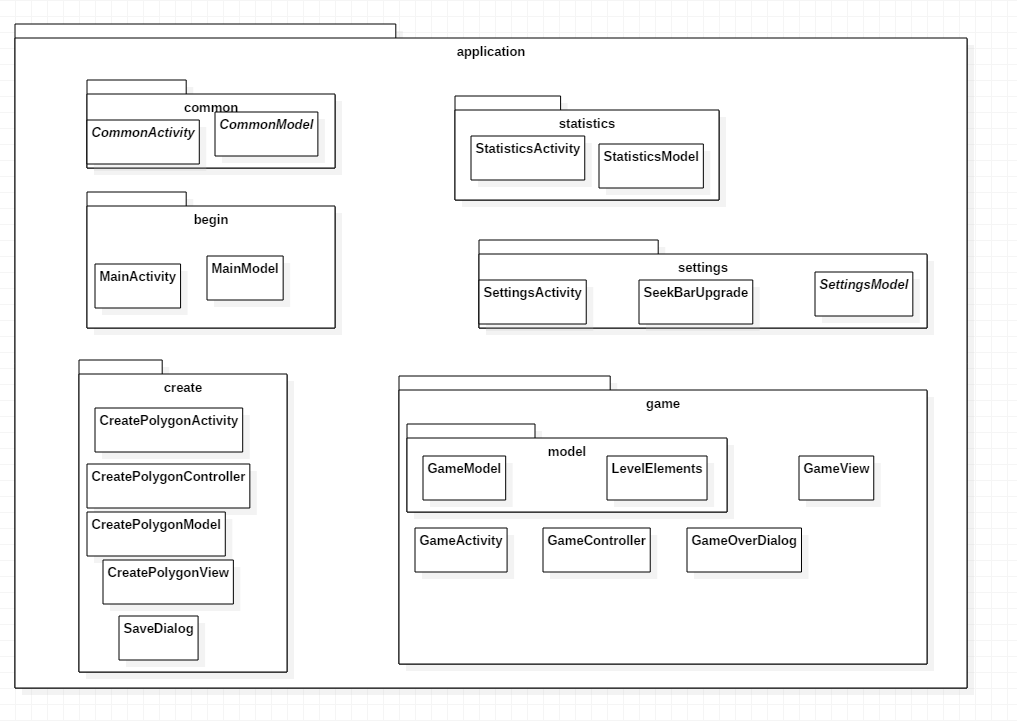
\includegraphics[scale=.7]{pictures/UML/package/application}
\caption{Организација класа по пакетима (application пакет)}\label{fig:umlPackageApp}
\end{center}
\end{figure}

\begin{figure}[htb!]
\begin{center}
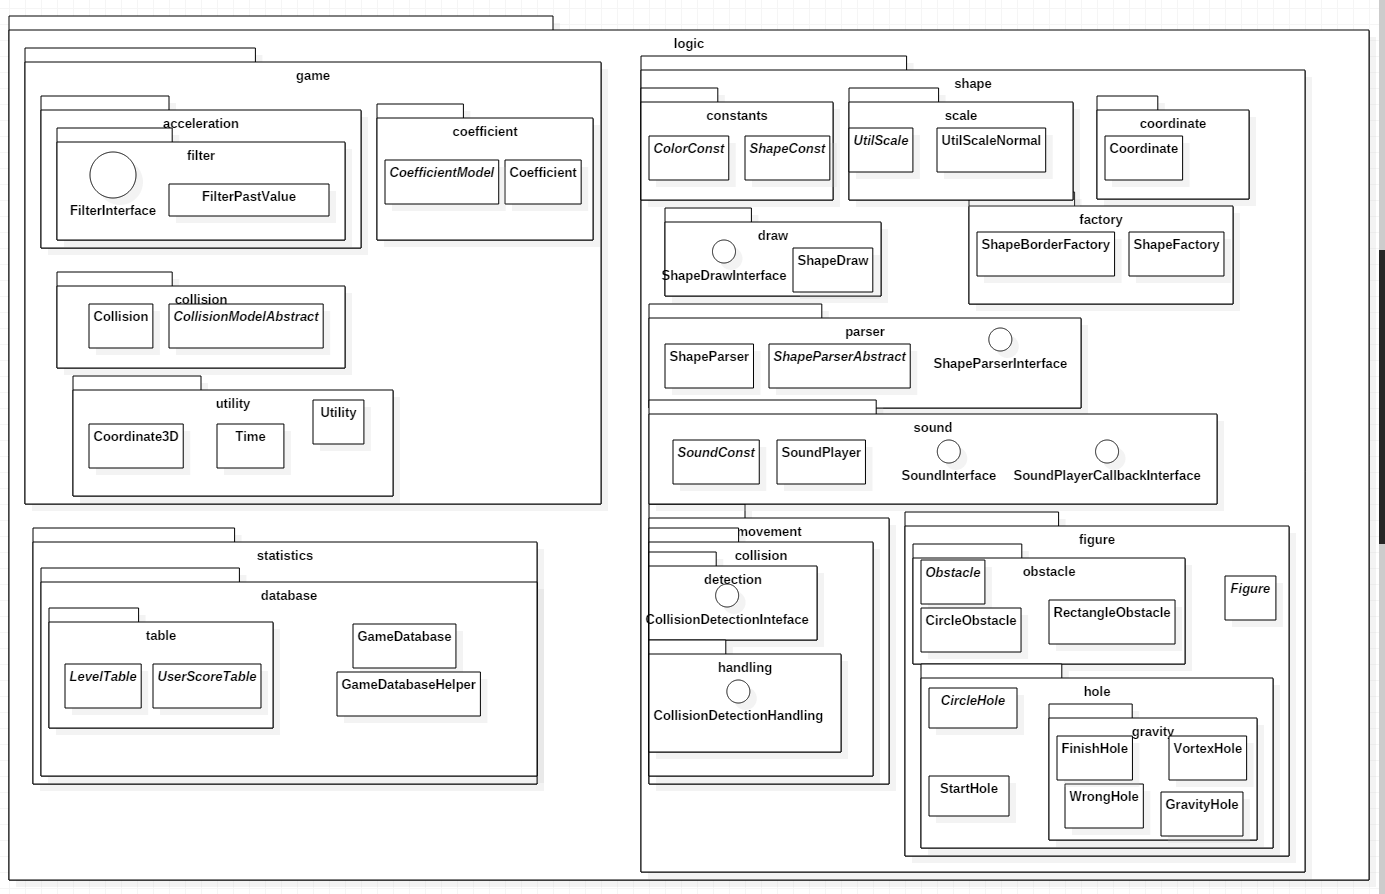
\includegraphics[scale=.6]{pictures/UML/package/logic}
\caption{Организација класа по пакетима (logic пакет)}\label{fig:umlPackageLog}
\end{center}
\end{figure}

Читав java код је организован тако да се налази унутар пакета \emph{com.example.popina.projekat} и то у два потпакета. Код који је везан за MVC преглед и Android део налази се у applicatiоn потпакету (слика \ref{fig:umlPackageApp}). Код који је везан за логику игре (база података, како се праве фигуре, парсира...) налази се у потпакету logic (\ref{fig:umlPackageLog}). Логика класа из потпакета application је објашњена у глави \ref{Android}, као и у глави \ref{Graphics}. Такође логика пакета \emph{coefficent} je објашњена у глави  \ref{Android}, као и логика \emph{collision} пакета унутар кога је \emph{collisionMode}l. Стога овде ће бити објашњена организација кода у потпакету logic који описује логику тј. како ради апликација. 

\section{Пакет game}
\subsection{Пакет acceleration.filter}

\begin{figure}[htb!]
\begin{center}
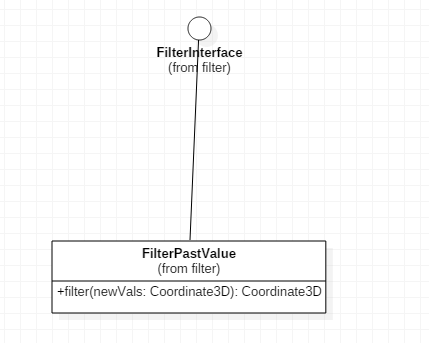
\includegraphics[scale=.6]{pictures/UML/class/filter}
\caption{Класа filter}\label{fig:umlClassFilter}
\end{center}
\end{figure}

Унутар овог пакета се налази интерфејс \emph{FilterInterface} чија метода \emph{filter} прима очитане вредности убрзања са улаза и враћа филтриране вредности. Ово спречава да се дешавају нагле промене убрзања услед случајно лошег очитавања сензора. У апликацији је имплементирана у виду \emph{FilterPastValue} класе (слика \ref{fig:umlClassFilter}).Ова класа филтрира тако што последњу филтрирану вредност и ону детектовану скалира тако да $\alpha$($0 \leq \alpha \leq 1$) се множи са новом вредношћу, а са $1-\alpha$ са старом и то се сабира. Ова класа се користи код филтрирања вредности убрзања у \emph{GameActivity}. 

\subsection{Пакет coefficient}
У овом пакету класа \emph{Coefficient} са методом \emph{updateValues} чува коефицијенте унутар \emph{SharedPreferences} (чије име се налази у \emph{CoefficientModel}). 
\subsection{Пакет collision}
Класа \emph{CollisionModelAbstract} има методу \emph{updateSystem} која прима за аргументе филтрирано убрзање. време детекције сензора, листу  \emph{Figure} којe представљају препреке, или циљ за лопту, као и саму лопту. Након позива ове методе треба да буде ажурирана позиција лопте, као и пуштен одговарајући звук player-ом који је примила класа у конструктору. Враћа једну од 4 вредности које кажу да ли је игра побеђена, изгубљена, да ли има колизије или нема колизије. Метода \emph{setLastTime} служи за иницијализцију референтног времна од кога ће мерити промена брзине лопте.
\subsection{Пакет utility}
Овде се садрже како само име каже Utility ствари као што су \emph{Coordinate3D} која представља 3D координату тачке у простору. \emph{Time} која представља временски интервал која има почетак и крај и чија дужина може да се рачуна преко методе \emph{timeInt}.  
\\ \indent 
Класа \emph{Utility} обухвата методе које служе за рад са координатама, конверзијама, насумичним бројем. Метода \emph{radianToDeg} претвара угао из радијана у степене. Meтода \emph{degToRadian} претвара угао у степенима у радијане.  Метода \emph{convertMsToS} претвара из милисекунди у секунде, док \emph{convertNsToS} претвара из наносекунди у секунде. Метода \emph{opositeSign }враћа супротан знак од броја који је прослеђен. Метода \emph{convertRadianAngleTo2PiRange} пребацује угао у радијанима у $\left[ o, 2 \pi \right]$ интервал. Метода \emph{randomNumberInInterval} враћа број у задатом интервалу. Meтода \emph{rotatePointAroundCenter} ротира тачку око центра за одређени угао (тамо где нема центра узима се $(0, 0)$ за центар, тамо где нема угла користе се израчунате вредности синуса и косинуса које су прослеђене за брже рачунање ротацје). \emph{calculateAngle} рачуна угао између $x$ осе и праве одређене тачком и центром. Метода \emph{doesSegmentIntersectsCircle}одређује да ли круг сече прослеђени сегмент, са тим да су сегменти увек паралелни $x$ или $y$ оси што се прослеђује последњи параметром. Метода \emph{isDimBetweenDims} одређује да ли је вредност између две вредности на реалној правој, при чему се користи одступање од $0,01$. \emph{distanceSquared} враћа растојање између две координате квадрирано. \emph{isDistanceBetweenCoordLesThan} Одређује да ли је растојање између две координате мање од прослеђеног, при чему се користи тачност од $0,01$. Aко јe растојање већ квадрирано нема потребе да се квадрира (што се може проследити као параметар).